\section{Preliminary work}
\subsection{Estimating two-dimensional elastic moduli}
The motivation for Specific Aims 1-3 stemmed from the successful demonstration of gradient driven
self-assembly of amphiphilic particles into two-dimensional micelles,
bilayer membranes, \cite{Fu2018_SIAM}, and recreation of the vesicles tank-treading phenomenon.

Our preliminary work on membrane elasticity 
is particulary encouraging because the effective bending, stretch, and tilt elastic moduli we calculated
were in excellent agreement with the experimental values (Table \ref{tab:moduli}).
The agreement is underscored by the fact we assigned reasonable physical values to 
the main model parameters of HAP energy, rather than tuning parameters.

\begin{table}[h!]
\begin{center}
  \begin{tabular}{|l|p{0.16\textwidth}|l|l|p{0.2\textwidth}|p{0.18\textwidth}}
    \hline
          & simulation type & HAP value        & experimental value & reference\\
    \hline \hline 
    $\KB$ & {\footnotesize uniform load with clamped condition} & $11 \pm 2.5$ \kBT & 10 \kBT                  & \cite{Naetal15,VeBrPa15,NAGLE2000159,PhysRevLett.113.248102}\\
    \hline 
    $\KA$ & {\footnotesize bilayer stretching}  & $34$ \kBT $^{-2}$ & 30--40 \kBT $^{-2}$              & \cite{Nagle17, Nagle17-2}\\
    \hline 
    $\KTH$ & {\footnotesize tilt Dirichlet condition} & $12$ \kBT \; nm$^{-2}$ & 10 \kBT $^{-2}$  &  \cite{KUZMIN2005, KoNa15} \\ \hline
  \end{tabular}
\end{center}
\caption{\label{tab:moduli}Comparision of values elastic moduli from the experimental literature and values derived by HAP simulation.}
\end{table}



\subsection{Two-dimensional vesicle hydrodynamics in shear flow} 
%The motion of vesicles in shear flow is an important
%problem in the applied mathematics because simulations can reveal mechanical
%properties of membranes and lead to an enhanced understanding of 
%deformable particle laden flows \cite{Sinha15}. 
%
%
\begin{wrapfigure}[10]{r}{0.2\textwidth}
\centerline{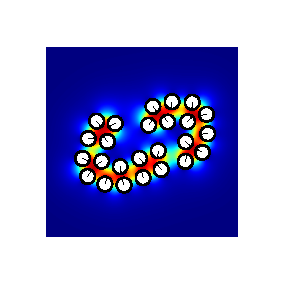
\includegraphics[width=0.2\textwidth]{figures/PW_fig5.pdf}}
\vspace{-8pt}
\caption{\label{fig:rupture} \footnotesize Rupture of tank-treading vesicle under strong shear flow.}
\end{wrapfigure}
%
To implement a vesicle in shear flow in the context of hydrophobic
potentials and mobility problem, we consider a shear flow in the
far-field $\mathbf{u}_{\infty} = Uy\mathbf{i}_x$ in the direction of the
$x$-axis (Figure \ref{fig:tanktreading}A). As illustrated in Figure
\ref{fig:tanktreading}, the particle based approach supports
inter-leaflet slip, and this can be used to determine inter-leaflet and
in-plane shear viscosities. 
%
%This field satisfies the linear Stokes system but does not give rise to a rigid motion at the particle interfaces. 
%To have a rigid motion, we change variables $\mathbf{u} = \tilde{\mathbf{u}}+ \mathbf{u}_{\infty}$ and 
%for the new field $\tilde{\mathbf{u}}$ vanishing at infinity we let 
%$\tilde{\mathbf{u}}|_{\partial P_i} = \mathbf{v}_i + \boldsymbol{\omega}_i \times (\mathbf{x} - \mathbf{a}_i)$ 
%where $(\mathbf{v}_i,\boldsymbol{\omega}_i)$ are the unknown translation and angular velocities of the 
%$i$th particle $P_i.$  
%
%\begin{wrapfigure}[17]{l}{0.4\textwidth}
%\centerline{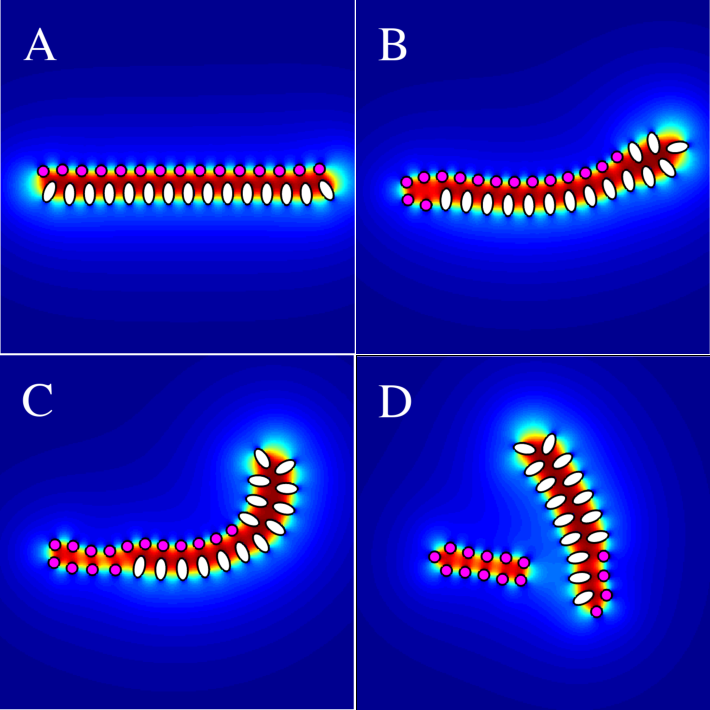
\includegraphics[width=0.4\textwidth]{figures/PW_fig2.pdf}}
%\caption{\label{fig:demixing} An initial assembly of small and 
%large particles spontaneous segregates into two smaller bodies. }
%\end{wrapfigure}
The HAP simulations show vesicle tank-treading. Under the external shear flow, the initially circular 
vesicle rotates in the clockwise direction. As the rate of rotation increases, the vesicle approaches
a steadily tank-treading ellipse. In Figure \ref{fig:tanktreading}B-D, the solid curves are ellipses fit to the particle centers
and midplane respectively. In the non-dimensionalized system, the particles have diameter 2, on the order of $\rho,$ 
and the vesicle diameter is about 14. 
%\todo[inline]{missing units. nm?}
Figure~\ref{fig:tanktreading}E shows the aspect ratio of the major to minor axes reaching an equilibrium value in the 
red and blue curves, yet oscillating in the high-shear rate (yellow) curve.
The tank-treading vesicle elongates and becomes more horizontal 
with an increase in flow rate or 
with a decrease in stiffness (effected by decreasing $\rho = 4$ to $\rho = 2$). 


For large shear flow rates, there is an increase in arc length. Here arc
length refers to the the mid-plane circumference. Thus, some of the
external force is going into stretching the vesicle---the other part is
going into bending and viscous dissipation. From our experiments, we
find that the vesicle ruptures once stretching exceeds about 5 \% (see
Figure \ref{fig:rupture}). Finally, movies of the tank-treading motion
show a slip velocity between the outer and inner leaflets Figure
\ref{fig:tanktreading}G. We have illustrated this by tracking the
distance between two reference particles in the inner and outer leaflet
(Figure \ref{fig:tanktreading}B \& D, green and blue particles). With
moderate shear rates or greater adhesion, the particle pair moves in
tandem (in Figure \ref{fig:tanktreading}H, blue and red curves, their
distance is more or less constant). For a large shear rate, the
particle separates as the two leaflets slide against one another. 

\begin{figure}
\begin{center}
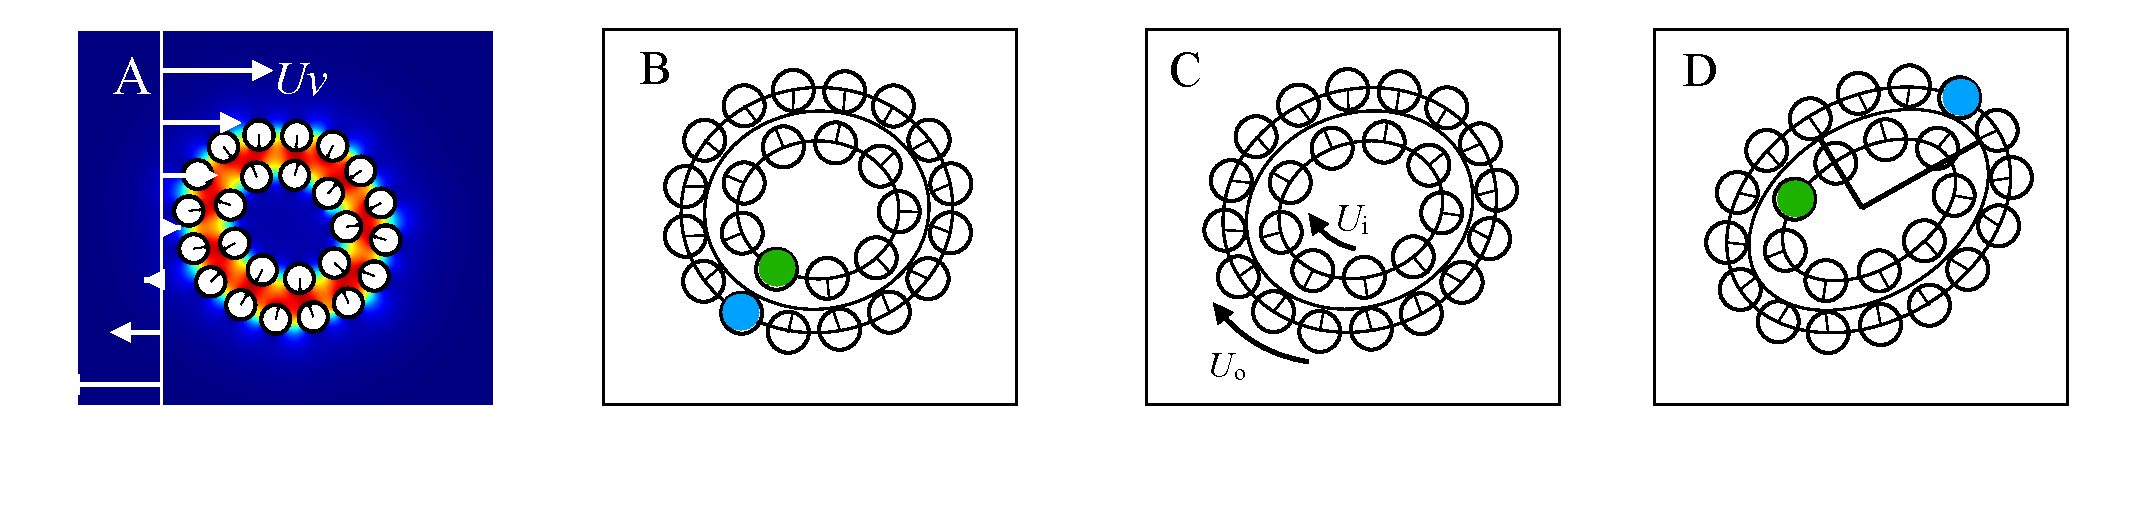
\includegraphics[width=1\textwidth]{figures/PW_fig1A-D.pdf}
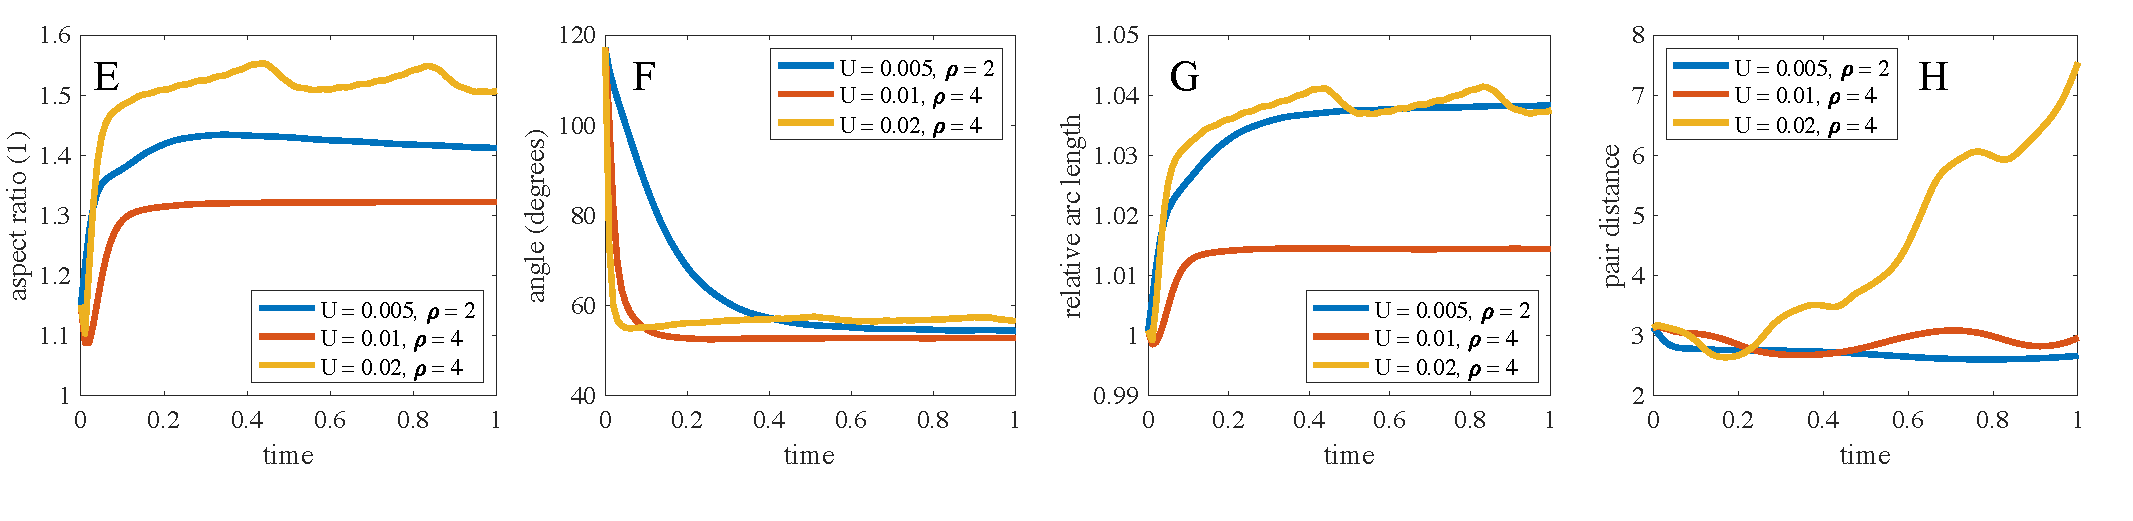
\includegraphics[width=1\textwidth]{figures/PW_fig1E-H.pdf}
\end{center}
\vspace{-0.3in}
\caption{\label{fig:tanktreading}\footnotesize (A) A vesicle formed by
  amphiphilic particles in shear flow, and the tank-treading motion
  (B)--(D). The separation of particle pairs in (B) and (C) illustrate
  inter-leaflet slip.  (E)--(G) Tank-treading reaches a steady state in
  elliptical aspect ratio, major-axis angle, and circumference.}
\end{figure}


%\begin{wrapfigure}[12]{r}{0.2\textwidth}
%\centerline{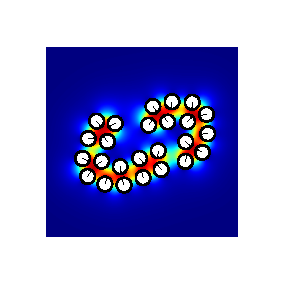
\includegraphics[width=0.2\textwidth]{figures/PW_fig5.pdf}}
%\caption{\label{fig:rupture} Rupture of tank-treading vesicle under strong shear flow.}
%\end{wrapfigure}
%




